% Copyright 2004 by Till Tantau <tantau@users.sourceforge.net>.
%
% In principle, this file can be redistributed and/or modified under
% the terms of the GNU Public License, version 2.
%
% However, this file is supposed to be a template to be modified
% for your own needs. For this reason, if you use this file as a
% template and not specifically distribute it as part of a another
% package/program, I grant the extra permission to freely copy and
% modify this file as you see fit and even to delete this copyright
% notice. 

\documentclass{beamer}
\usepackage{amsmath}
\usepackage{bm}
% There are many different themes available for Beamer. A comprehensive
% list with examples is given here:
% http://deic.uab.es/~iblanes/beamer_gallery/index_by_theme.html
% You can uncomment the themes below if you would like to use a different
% one:
%\usetheme{lankton-keynote}
%\usetheme{AnnArbor}
%\usetheme{Antibes}
%\usetheme{Bergen}
%\usetheme{Berkeley}
%\usetheme{Berlin}
%\usetheme{Boadilla}
%\usetheme{boxes}
%\usetheme{CambridgeUS}
%\usetheme{Copenhagen}
%\usetheme{Darmstadt}
%\usetheme{default}
%\usetheme{Frankfurt}
%\usetheme{Goettingen}
%\usetheme{Hannover}
%\usetheme{Ilmenau}
%\usetheme{JuanLesPins}
%\usetheme{Luebeck}
\usetheme{Madrid}
\usepackage[final]{pdfpages}
%\usetheme{Malmoe}
%\usetheme{Marburg}
%\usetheme{Montpellier}
%\usetheme{PaloAlto}
%\usetheme{Pittsburgh}
%\usetheme{Rochester}
%\usetheme{Singapore}
%\usetheme{Szeged}
%\usetheme{Warsaw}
%\usecolortheme{beetle}

\newcommand*\samethanks[1][\value{footnote}]{\footnotemark[#1]}

\setbeamertemplate{navigation symbols}{}%remove navigation symbols
\title[The Network of FDI Flows]{The Network of Foreign Direct Investment Flows:\\Theory and Empirical Analysis\thanks{\footnotesize {Acknowledgement: This material is based on work supported by the National Science Foundation under IGERT Grant DGE-1144860, Big Data Social Science.}}}


\author[J.\,Schoeneman, B. \,Zhu \& B.\,Desmarais]{%
  \texorpdfstring{%
    \begin{columns}
      \column{.3\linewidth}
      \centering
      John Schoeneman{\thanks{Pennsylvania State University}} \\ \small{jbs5686@psu.edu\\ PhD Candidate}
      \column{.3\linewidth}
      \centering
      Boliang Zhu{\samethanks[2]} \\ \small{bxz14@psu.edu\\ Assistant Professor}
    \end{columns}
    \vspace{12pt}
    \begin{columns}
      \column{.3\linewidth}
      \centering
      Bruce Desmarais{\samethanks[2]}\\ \small{bdesmarais@psu.edu\\ Associate Professor}
    \end{columns}
 }
 {Author 1, Author 2, Author 3}
}

\date{April 8, 2017}



% - Use the \inst command only if there are several affiliations.
% - Keep it simple, no one is interested in your street address.

% - Either use conference name or its abbreviation.
% - Not really informative to the audience, more for people (including
%   yourself) who are reading the slides online


% This is only inserted into the PDF information catalog. Can be left
% out. 

% If you have a file called "university-logo-filename.xxx", where xxx
% is a graphic format that can be processed by latex or pdflatex,
% resp., then you can add a logo as follows:

% \pgfdeclareimage[height=0.5cm]{university-logo}{university-logo-filename}
% \logo{\pgfuseimage{university-logo}}


% Let's get started
\begin{document}

\begin{frame}
  \titlepage
\end{frame}


% Section and subsections will appear in the presentation overview
% and table of contents.


\begin{frame}{Introduction}

\frametitle{Introduction}
  \begin{columns}[T]
    \begin{column}{.5\textwidth}
\vspace{10mm}
\begin{itemize}
\item{FDI as a Network}
\begin{itemize}
\item{Clustering}
\item{Reciprocity}
 \end{itemize}
 \item{Motivation}
 \begin{itemize}
\item{Violation of Independence Assumptions}
\item{Theoretical Importance of Dependence Terms}
 \end{itemize}
  \item{Simultaneously test exogenous variables as well}
 \end{itemize}
    \end{column}
    \begin{column}{.5\textwidth}
    \begin{block}{FDI Network 2008}
    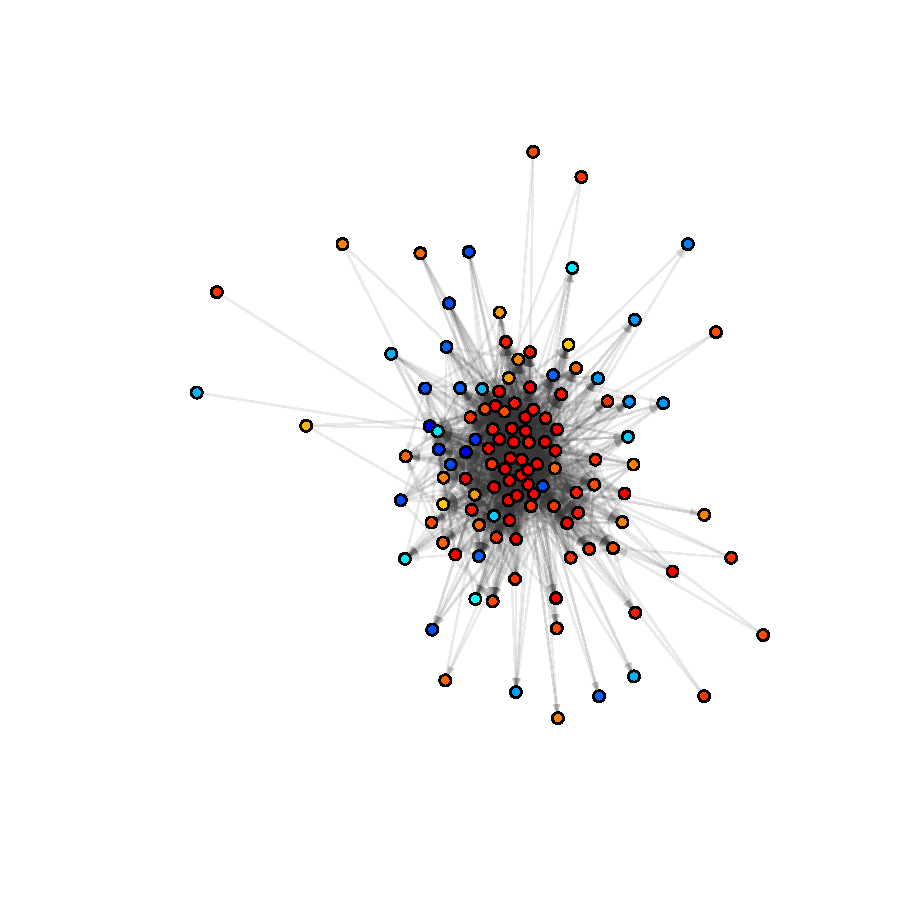
\includegraphics[scale=.4]{slides_figures/fdiNet2008.pdf}
 \small{\\ Color Scheme: Autocracy to Democracy is scaled as Blue to Red}
    \end{block}
    \end{column}
  \end{columns}

%In the image on the right is the network for weighted FDI flows for 2008. There are a couple things that are immediately obvious. The first is that we clearly see clustering. This clustering is based on FDI flows, which are the ties for between nodes, which here are countries. The more ties a node has and the larger these ties are, the more centrally placed a node is and the more shared partners and size of edge they share with a node, the closer they are to that node. This clear dependence in structure motivates us to model these networks, both to eliminate the potential bias that comes from ignoring them and measure the dependence, which we argue has theoretical importance. The second point is that it appears Polity plays a role in clustering as well, with red, democratic nodes often close to one another. Network models allow us to test exogenous variables such as the role of regime type alongside of network terms, and so we focus on both political and economic variables that have been estimated in the past, but in standard regression models that assumed independence.

\end{frame}

\begin{frame}{Theory for Network Terms}
\begin{columns}[T]
    \begin{column}{.5\textwidth}

\begin{itemize}
\item{Reciprocity}
\begin{itemize}
\item{Standard practice to resolve political opposition from competing firms}
\item{Anti-reciprocal relationship in mixed dyads}
\end{itemize}
\end{itemize}
\vspace{10mm}
\begin{itemize}
\item{Transitivity}
\begin{itemize}
\item{MNC expansion and supply-chain fragmentation}
\item{Risk of Expropriation}
\item{PTA networks}
\end{itemize}
\end{itemize}
    \end{column}
    \begin{column}{.5\textwidth}
    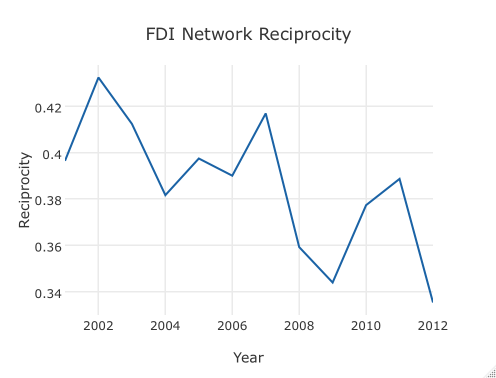
\includegraphics[scale=.3]{slides_figures/reciprocity.png}\vfill
    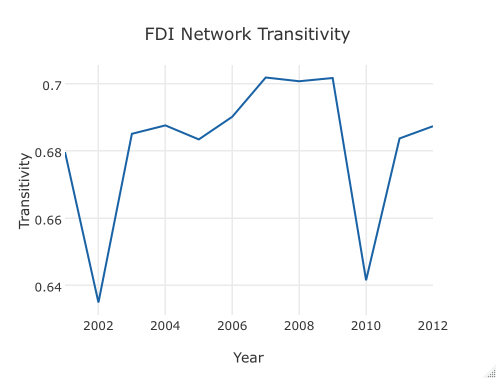
\includegraphics[scale=.3]{slides_figures/transitivity.png}
        \end{column}
  \end{columns}
% We focus on two network dependencies in our model and provide theoretical reasons for them. The first is reciprocity. In the figure to the right we see that weighted reciprocity, scaled between -1 and and 1, is present. As with trade, expansion of a foreign firm into country's market is generally met with some opposition by the owners of similar firms. The political way to resolve this conflict is through reciprocal agreements. This can placate the host country MNCs by granting them or other firms access to new markets to built up sufficient political support for the MNCs. However, it is important to note the this behavior best explains the relationship between developed countries that have competing MNCs, whereas mixed dyads are more likely to be anti-reciprocal. This is not explored in the models, but will be addressed in future work. However, there is some evidence of this in the decline of reciprocity over time as more and more FDI is vertical and between mixed dyads.
% The second network dependency is transitivity, or the clustering coefficient. In the figure to the right, unweighted and undirected transitivity, calculated as the number of triadic closures for all possible triads where a two-path exists, the percentage is quite high. Global production supply chains are increasingly complex and disaggregated. With large MNCs being the dominant players, they often invest in multiple countries for one finished product, and are increasingly involved in all levels of production, which increases the chance that an investor is more likely to invest in a country for which a two-path already exists. Also, since there is inherent risk in investment, that is the possibility of expropriation of fixed investments, investment is encouraged to cluster along particular countries that have a sustained interest in protecting investors, leading to triadic closures in the network. Another key factor is that this FDI is vertical and thus dependent on trade liberalization. PTAs then can reinforce or expand these triadic clusters through the expansion of trade networks. 

\end{frame}

\begin{frame}{FDI Data and Exogenous Covariates}

\begin{itemize}
\item{Bilateral FDI statistics from UNCTAD, 2001-2012}
\end{itemize}

\begin{columns}[T]
    \begin{column}{.5\textwidth}
\begin{itemize}
\item{Dyad-level Covariates}
\begin{itemize}
\item{Gravity +} 
\item{Contiguity +} 
\item{Common Language +} 
\item{Four Types of Defense Treaties +}  
\item{Colonial Relationships +}
 \item{PTA depth$^{1}$ + }
\end{itemize}
\end{itemize}
    \end{column}
    \begin{column}{.5\textwidth}
\begin{itemize}
\item{Node-level Covariates}
\begin{itemize}
\item{GDP per capita +/-} 
\item{GDP Growth Rate +} 
\item {Polity IV +} 
\item{Political Violence - } 
\item{Trade Openness +}
\end{itemize}
\end{itemize}
        \end{column}
  \end{columns}
 
 %Our dependent variable is from recently made available data from UNCTAD. It covers 2001 to 2012. We use FDI stock levels since we take the log and FDI stock has fewer negative values. Although, we include a lagged dependent variable, so our covariates are estimating remaining variation, which is FDI flows.  
  
%Dyad: Alongside the network terms we estimate size dyad level relationship. We begin with gravity variables , which have been the workhorse in the trade and FDI literature. Gravity variables include the logged product of the dyad's GDPs and the logged euclidean distance. Binary variables in the model include contiguity, defense treaties, common language, and former colonial ties, for which we expect positive correlations. The last dyad level covariate is PTA depth, which we argue is related to transitivity. This depth variable comes from a recent dataset that used 48 different dichotomous variables, such as trade in services, SPS measures, etc., to create a latent measure of agreement depth.

%Node: We also include five node level covariates, which we estimate both their relationship with receiving FDI and sending FDI.  GDP per capita represents factor endowments for a country. If FDI mainly flows from capital rich countries to labor rich countries, we expect it to be positive for the origin node and negative for the destination node. Growth rate, as a proxy for general economy health, should be positive for both directions. Literature for the democracy score, using the common Polity IV measure, is inconclusive, but there is a general expectation that better institutions will attract more FDI. Political Violence, which can inversely proxy for political stability, can proxy for regime stability, which is important for investors to consider since a change in government can result in new investment conditions, and thus we expect to be negatively related to FDI flows for both directions. Trade openness would be positive for both directions given the complementary relationship between trade and FDI. 

\end{frame}


\begin{frame}{ERGM Count Model}

\small{

$$ \text{Pr}_{\bm{\theta};h;\bm{g}}( \bm{Y}=\bm{y} )=\frac{ h(\bm{y})\text{exp}( \bm{\theta} \cdot \bm{g} (\bm{y}) )}{\bm{\kappa}_{h,\bm{g}}(\bm{\theta})} $$

$$\text{Sum}:\bm{g(y)} = \sum_{(i,j) {\in} \mathbb{Y}}\bm{y}_{i,j}$$

$$\text{Sum, Fractional Moment}:\bm{g(y)} = \sum_{(i,j) {\in} \mathbb{Y}}\bm{y}_{i,j}^{1/2}$$

$$\text{Non-Zero}: \bm{g}_k = \sum_{(i,j) {\in} \mathbb{Y}} \mathbb{I}(\bm{y}_{i,j} \neq 0)$$

$$ \text{Reciprocity}: \bm{g(y)} = \sum_{(i,j) {\in} \mathbb{Y}}min(\bm{y}_{i,j},\bm{y}_{j,i})$$

$$\text{Transitive Weights}: \bm{g(y)} =  \sum_{(i,j) {\in} \mathbb{Y}}\min\bigg( \bm{y}_{i,j}, \max\limits_{k{\in}N}\Big(\min(\bm{y}_{i,k},\bm{y}_{k,j})\Big) \bigg),$$ 

$$ \text{Dyadic Covariate}: \bm{g(y,x)} = \sum_{(i,j)} \bm{y}_{i,j}x_{i,j}$$ 

$$ \text{Sender Covariate}: \bm{g(y,x)} = \sum_{i}x_i \sum_{j} \bm{y}_{i,j}$$

$$ \text{Receiver Covariate}: \bm{g(y,x)} = \sum_{j}x_j \sum_{i} \bm{y}_{i,j}$$

}

%where $\bm{g}( \bm{y} )$ is the vector of network statistics used to specify the model, $\bm{\theta}$ is the vector of parameters that describes how those statistic values relate to the probability of observing the network, $h(\bm{y})$ is a reference function defined on the support of $\bm{y}$ and selected to affect the shape of the baseline distribution of dyadic data (e.g., Poisson reference measure), and $\bm{\kappa}_{h,\bm{g}}(\bm{\theta})$ is the normalizing constant that assures that the probabilities over all possible networks sums to one. 

%average edge value and dispersion in the edge distribution

%which models the prevalence of zeros in dyadic FDI flows. 

%in which we add up the lowest edge value within each dyad. If edges are reciprocated, this statistic will increase due to the co-occurrence of large edge values within the same dyad. 

% which acounts for the degree to which edge $(i,j)$ co-occurs with pairs of large edge values with which  edge $(i,j)$ forms a transitive (i.e., non-cyclical) triangle. 


% measures this co-occurrence at the level of the directed dyad, in which there is a dyadic observation of the covariate corresponding to each potential FDI flow. 

%Each statistic takes the product of the node's covariate value and a sum of the edge values in which the node is involved. The first, ``Sender Covariate,'' uses the sum over the flows that the node sends. The second, ``Receiver Covariate,'' uses the sum over the flows that the node receives. These two variants of node-level statistics differentiate between the effects of a variable on the volume of FDI originating from a state, and being invested in a state, respectively.



%\noindent The count ERGM estimates that we present below are estimated using the \texttt{ergm} \citep{ergm} and \texttt{ergm.count} \citep{ergmcount} packages in the \R \space statistical software \citep{r}.



% General explanation of ERGM
	% How does this solve the problem of dependences
% How network terms are estimated
% How Exogenous Variables are included

\end{frame}


\begin{frame}{Count Model and Network Dependencies}

% Network measurements and what they mean

\end{frame}



\begin{frame}{Covariate Results}

% Model Specfication

\end{frame}


\begin{frame}{Conclusion and Future Research}

\end{frame}


\begin{frame}{References}
\begin{enumerate}
\item{D{\"u}r, A., Baccini, L., \& Elsig, M. (2014). The design of international trade agreements: Introducing a new dataset. The Review of International Organizations, 9(3), 353-375.}
\end{enumerate}
\end{frame}




\end{document}




